\chapter{Beam tests}\label{chap::6}

\vfill

\minitoc

\newpage

\glsresetall
\glsunset{clarys} 


As described in chapter~\ref{chap::3}, the components of the \gls{clarys} gamma cameras are at the final characterization phase, and the efforts of the collaboration are presently mainly focused on the optimization of the acquisition chain, including the electronics boards, the \gls{utca} acquisition system and the associated acquisition, monitoring and slow control software. These tasks foresee several measurements campaigns, and three of them have been performed between the end of 2017 and the date of writing (September 2018), and are presented in this chapter. 
All the presented beam tests have been carried out at the \gls{cal} in Nice with a 65~MeV proton beam. The Nice hadrontherapy platform was the first site in France starting to treat patients in June 1991 with the MEDYCIC cyclotron proton beams. The cyclotron was designed to support regular neutron and proton therapy programs, as well as for the production of $^{18}$F for \gls{pet} applications~\parencite{Mandrillon1989, Mandrillon1992}. The accelerator is a fixed frequency 25~MHz isochronous cyclotron with a peak voltage of 50kV. Negative hydrogen ions are produced by an external source, axially injected and accelerated to 65~MeV. The extraction is performed by a 60$\times$10$^{-6}$ g/cm$^2$ carbon stripping foil and the exiting protons are transported down the beam line to the treatment room~\parencite{Herault2005}, or to the research nozzle used for the presented beam tests. The layout of the MEDICYC facility is shown in \figurename~\ref{chap6::fig::MEDICYC_layout}.

 \begin{figure}[!htbp]
\centering
\includegraphics[width=0.6\textwidth]{03_GraphicFiles/chapter6_BeamTests/MEDiCYC.pdf}
\caption{Layout of the Nice MEDICYC facility. In~\cite{Mandrillon1992}.}
\label{chap6::fig::MEDICYC_layout}
\end{figure}



\section{Hodoscope: december 2017}

\section{Hodoscope: may 2018}


\begin{figure}[!htbp]
\centering
\includegraphics[width=0.5\textwidth]{03_GraphicFiles/chapter6_BeamTests/Nice_May2018/scheme.png}
\caption{}
\label{chap6::fig::May_HodoDAQscheme}
\end{figure}

\begin{figure}[!htbp]
\centering
\includegraphics[width=0.8\textwidth]{03_GraphicFiles/chapter6_BeamTests/Nice_May2018/map2D.pdf}
\caption{}
\label{chap6::fig::May_HodoMap2D}
\end{figure}


\begin{figure}
\begin{subfigure}[b]{.5\textwidth}
\centering
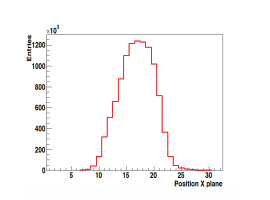
\includegraphics[width=0.9\textwidth]{03_GraphicFiles/chapter6_BeamTests/Nice_May2018/profileX.png}
\caption{}
\label{chap6::fig::May_HodoprofX}
\end{subfigure}
\begin{subfigure}[b]{.5\textwidth}
\centering
\includegraphics[width=0.9\textwidth]{03_GraphicFiles/chapter6_BeamTests/Nice_May2018/profileY.png}	
\caption{}
\label{chap6::fig::May_HodoprofY}
\end{subfigure}
\caption{}
\label{chap6::fig::May_Hodoprof1D}
\end{figure}

\begin{figure}
\begin{subfigure}[b]{.5\textwidth}
\centering
\includegraphics[width=0.9\textwidth]{03_GraphicFiles/chapter6_BeamTests/Nice_May2018/clusterX.png}
\caption{}
\label{chap6::fig::May_HodoClusX}
\end{subfigure}
\begin{subfigure}[b]{.5\textwidth}
\centering
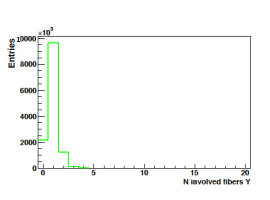
\includegraphics[width=0.9\textwidth]{03_GraphicFiles/chapter6_BeamTests/Nice_May2018/clusterY.png}	
\caption{}
\label{chap6::fig::May_HodoClusY}
\end{subfigure}
\caption{}
\label{chap6::fig::May_HodoClusters}
\end{figure}

\begin{figure}
\begin{subfigure}[b]{.5\textwidth}
\centering
\includegraphics[width=0.9\textwidth, trim={0 0.6cm 0 0} , clip=true]{03_GraphicFiles/chapter6_BeamTests/Nice_May2018/TX-Ttrig.png}
\caption{}
\label{chap6::fig::May_HododTx}
\end{subfigure}
\begin{subfigure}[b]{.5\textwidth}
\centering
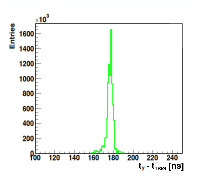
\includegraphics[width=0.9\textwidth]{03_GraphicFiles/chapter6_BeamTests/Nice_May2018/TY-Ttrig.png}	
\caption{}
\label{chap6::fig::May_HododTy}
\end{subfigure}
\caption{}
\label{chap6::fig::May_HodoDeltaT}
\end{figure}


\begin{figure}[!htbp]
\centering
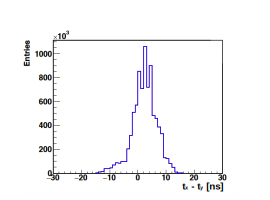
\includegraphics[width=0.6\textwidth]{03_GraphicFiles/chapter6_BeamTests/Nice_May2018/TX-TY.png}
\caption{}
\label{chap6::fig::May_HodoDeltaTFibers}
\end{figure}



\section{Collimated camera: september 2018}


\clearpage
%\printbibliography[heading=subbibintoc]
